\documentclass[journal,10pt,twocolumn]{IEEEtran}

\usepackage{cite}
\usepackage{amsmath,amssymb,amsfonts}
\usepackage{algorithmic}
\usepackage{graphicx}
\usepackage{textcomp}
\usepackage{xcolor}
\usepackage{booktabs}
\usepackage{multirow}
\usepackage{tabularx}
\usepackage{url}
\usepackage{hyperref}
\usepackage{subcaption}

\hypersetup{
    colorlinks=true,
    linkcolor=blue,
    citecolor=blue,
    urlcolor=blue
}

\begin{document}

% -------------------------------------------------------------
% 1. TITLE
% -------------------------------------------------------------
\title{Multimodal AI-Based Prenatal Anemia Screening Using Clinical Data and Conjunctival Images}

\author{
    \IEEEauthorblockN{Research Team} \\
    \IEEEauthorblockA{Department of Biomedical Engineering and Health Informatics}
}

\maketitle

% -------------------------------------------------------------
% 2. ABSTRACT (150-250 words)
% -------------------------------------------------------------
\begin{abstract}
Prenatal anemia remains a pervasive maternal health disorder contributing to adverse pregnancy outcomes, including preterm delivery, maternal fatigue, low neonatal birth weight, and postpartum hemorrhage. Although laboratory-based venous blood testing via Complete Blood Count (CBC) is the diagnostic standard, its clinical utility in resource-limited rural clinics is constrained by invasive phlebotomy requirements, infrastructure deficits, and laboratory turnaround delays. Conversely, emerging non-invasive smartphone optical imaging of the palpebral conjunctiva often exhibits low sensitivity and vulnerability to lighting inconsistencies. To overcome these uni-modal shortcomings, this study presents an end-to-end multimodal screening framework combining structured hematological data with ocular and ungual image biometrics. The architecture integrates an Extreme Gradient Boosting (XGBoost) model trained on 103,221 clinical CBC records and maternal vitals, alongside a deep Residual Network (ResNet-18) fine-tuned on 7,041 clinical conjunctival and nail bed images. On held-out validation cohorts, the tabular branch achieved 99.95\% accuracy (AUC-ROC: 0.9999), while the computer vision branch achieved 94.46\% accuracy (AUC-ROC: 0.9873). A confidence-weighted multimodal late-fusion mechanism synthesizes these predictions to yield 98.85\% accuracy (AUC-ROC: 0.9981), demonstrating that multimodal consensus successfully mitigates single-modality optical failures. Furthermore, the model is integrated into an interactive clinical decision-support system offering automated WHO-aligned risk stratification and evidence-based nutritional guidelines. This provides an accurate, non-invasive triage solution for antenatal care.
\end{abstract}

% -------------------------------------------------------------
% 3. KEYWORDS (4-6)
% -------------------------------------------------------------
\begin{IEEEkeywords}
Prenatal Anemia, Multimodal Learning, Conjunctival Images, XGBoost, ResNet-18, Clinical Decision Support.
\end{IEEEkeywords}

% -------------------------------------------------------------
% 4. INTRODUCTION
% -------------------------------------------------------------
\section{Introduction}
\IEEEPARSTART{P}{renatal} anemia is an acute gestational pathology characterized by a quantitative deficiency in circulating erythrocytes or an abnormally low concentration of hemoglobin ($\text{HGB}$) to meet physiological fetal-maternal oxygen demands. According to World Health Organization (WHO) clinical thresholds, anemia during pregnancy is formally diagnosed when maternal venous hemoglobin drops below $11.0\text{ g/dL}$ ($10.5\text{ g/dL}$ in the second trimester) \cite{ethiopian_dhs2024, taye2026machine}. 

Maternal anemia represents a major global health challenge, affecting more than 40\% of expectant mothers worldwide, with the highest burden concentrated in low- and middle-income countries (LMICs). The clinical sequelae of untreated gestational anemia are severe: chronic maternal hypoxemia impairs placental nutrient transport, elevating the incidence of intrauterine growth restriction (IUGR), spontaneous preterm delivery, small-for-gestational-age neonates, and perinatal maternal mortality driven by postpartum hemorrhage \cite{scirep2024postdelivery}.

Conventional screening relies on invasive venipuncture phlebotomy followed by automated electronic hematology counters. However, in rural dispensaries and resource-constrained community clinics, reliable blood-based testing is frequently impeded by shortages of single-use needles, absent refrigeration for reagents, electrical instability, lack of certified laboratory technicians, and cultural phobias surrounding blood draws \cite{kato2024hemoglobin, ijmr2026inflammation}.

Artificial intelligence (AI) and computer vision offer transformative opportunities to overcome these hurdles. By analyzing microvascular pallor across mucosal and cutaneous vascular beds—specifically the palpebral conjunctiva of the lower eyelid and fingernail beds—deep neural networks can perform rapid, contactless, and non-invasive screening \cite{conjunctiva2023detection, vit_conjunctiva2025}. 

Despite promising proof-of-concept studies, existing AI research exhibits critical deficiencies when applied to maternal healthcare. Prior models have predominantly operated in disciplinary silos: studies either analyze public demographic/CBC survey databases without photographic validation \cite{ethiopian_dhs2024, taye2026machine}, or deploy optical convolutional networks trained on non-pregnant volunteers \cite{conjunctiva2023detection, kato2024hemoglobin}. Crucially, clinical field trials of smartphone camera screening in pregnancy revealed catastrophic sensitivity drops (as low as 23.8\%) due to gestational plasma expansion, hemodilution, and mucosal pigmentation variations \cite{niada2024cureus, wemyss2025smartphone}. 

What is fundamentally missing is an integrated framework that bridges non-invasive digital imaging with clinical risk factor analytics for pregnancy-specific screening. To resolve this gap, we develop, evaluate, and deploy a dual-branch multimodal AI architecture combining:
\begin{enumerate}
    \item A gradient-boosted decision tree pipeline (XGBoost) trained on clinical blood count parameters and maternal hemodynamic records.
    \item A transfer-learned deep residual network (ResNet-18) processing palpebral conjunctiva and nail bed photographs.
    \item A confidence-weighted multimodal late-fusion layer that synthesizes both streams into a consensus diagnostic risk score.
    \item An operational decision-support tool that maps model predictions directly to WHO clinical triage priorities and biochemical dietary protocols.
\end{enumerate}

% -------------------------------------------------------------
% 5. LITERATURE REVIEW / RELATED WORK
% -------------------------------------------------------------
\section{Literature Review}
Recent literature on machine learning for anemia detection can be classified into image-based non-invasive approaches and tabular clinical prediction models. Table \ref{tab:literature} provides a structured comparative summary of ten benchmark studies analyzed during this investigation.

Early image-based approaches confirmed that palpebral conjunctiva vascularization strongly correlates with systemic hemoglobin levels. Ahmed et al. \cite{conjunctiva2023detection} achieved 92.5\% classification accuracy using convolutional neural networks on 710 conjunctival images. Chen et al. \cite{vit_conjunctiva2025} applied Vision Transformers (ViT-B/16), reporting 98.47\% accuracy, while Kato et al. \cite{kato2024hemoglobin} demonstrated continuous hemoglobin regression ($R=0.86$). However, none of these cohorts evaluated expectant mothers, failing to account for gestational hemodilution.

When non-invasive mobile applications were deployed in clinical maternity cohorts, substantial diagnostic vulnerabilities emerged. The NiADA clinical validation study conducted by Sharma et al. \cite{niada2024cureus} revealed that while the mobile AI app maintained 90\% specificity, its diagnostic sensitivity collapsed to 23.8\% among pregnant women. Similarly, Wemyss et al. \cite{wemyss2025smartphone} tested smartphone colorimetry on 486 pregnant Indian women and observed a specificity of only 26.1\%, highlighting that skin undertones, lighting flux, and ocular pigmentation severely degrade standalone optical assessments.

Concurrently, tabular epidemiological models achieved high statistical power using demographic health surveys. Kassa et al. \cite{ethiopian_dhs2024} utilized Random Forest on Sub-Saharan African Demographic and Health Surveys (DHS), achieving 97.0\% accuracy. Taye et al. \cite{taye2026machine} applied XGBoost to 14,569 maternal records, recording an AUC of 0.95. Mukherjee et al. \cite{ijmr2026inflammation} demonstrated 95\% sensitivity when adjusting for systemic inflammation markers (CRP/Ferritin), and Moradi et al. \cite{scirep2024postdelivery} predicted postpartum hemoglobin drops using neural networks. Chayan et al. \cite{maternal_survey2024synthesis} highlighted the diagnostic value of maternal vitals during antenatal care. Nevertheless, tabular algorithms remain strictly reliant on invasive blood testing.

\begin{table*}[t]
\centering
\caption{Systematic Comparative Review of the 10 Benchmark Literature Studies}
\label{tab:literature}
\renewcommand{\arraystretch}{1.2}
\begin{tabularx}{\textwidth}{lp{3.4cm}p{3.2cm}p{2.6cm}p{3.2cm}p{3.3cm}}
\toprule
\textbf{\#} & \textbf{Study / Citation} & \textbf{Dataset(s)} & \textbf{Model(s)} & \textbf{Reported Results} & \textbf{Primary Clinical Limitation} \\
\midrule
1 & Ahmed et al. (2023) \cite{conjunctiva2023detection} & 710 conjunctival images & CNN + Logistic Reg. & Acc: 92.5\%, Sens: 90.0\% & Non-pregnant volunteers only; controlled lighting. \\
2 & Sharma et al. (2024) \cite{niada2024cureus} & 556 patients (51 pregnant) & Smartphone DL (NiADA) & Gestational Sens: 23.8\%, Spec: 90\% & Severe sensitivity drop in pregnancy; image-only. \\
3 & Kassa et al. (2024) \cite{ethiopian_dhs2024} & 14,500 SSA pregnant women & Random Forest & Acc: 97.0\%, F1: 93.0\% & Pure tabular; lacks non-invasive optical validation. \\
4 & Taye et al. (2026) \cite{taye2026machine} & 14,569 weighted DHS records & XGBoost & Acc: 87.0\%, AUC: 0.95 & Binary outcome; lacks photographic cross-modal input. \\
5 & Chen et al. (2025) \cite{vit_conjunctiva2025} & Conjunctival/scleral images & ViT-B/16 Transformer & Acc: 98.47\%, AUC: 0.99 & High compute demands; unvalidated in gestational cohorts. \\
6 & Kato et al. (2024) \cite{kato2024hemoglobin} & 250 conjunctival images & CNN Regression Head & Lab Hb correlation $R=0.86$ & Modest sample size; lacks pregnancy severity grading. \\
7 & Mukherjee et al. (2026) \cite{ijmr2026inflammation} & 3,604 NHANES + 381 Indian & Optimized Random Forest & Sens: 95.0\%, Spec: 95.0\% & Non-pregnant; requires complete invasive venipuncture. \\
8 & Moradi et al. (2024) \cite{scirep2024postdelivery} & 1,974 peripartum women & Artificial Neural Network & RMSE: 0.62 Hb & Single hospital cohort; lacks non-invasive screening. \\
9 & Wemyss et al. (2025) \cite{wemyss2025smartphone} & 486 pregnant Indian women & Colorimetric Modeling & Sens: 89.6\%, Spec: 26.1\% & Poor specificity due to skin pigmentation and ambient lux. \\
10 & Chayan et al. (2024) \cite{maternal_survey2024synthesis} & 1,205 gestational records & Statistical Profiling & Baseline diagnostic risk & Focuses on maternal vitals without computer vision fusion. \\
\midrule
\textbf{Ours} & \textbf{Proposed Study (2026)} & \textbf{104,400 tabular + 7,041 images} & \textbf{XGBoost + ResNet-18 Late Fusion} & \textbf{Tab: 99.95\%, Img: 94.46\%, Fused: 98.85\%} & \textbf{Eliminates single-modality bias via consensus triage.} \\
\bottomrule
\end{tabularx}
\end{table*}

% -------------------------------------------------------------
% 6. RESEARCH GAP
% -------------------------------------------------------------
\subsection{Research Gap}
Existing research focuses exclusively on either tabular laboratory prediction or photographic microvascular pallor analysis in isolation. Tabular models require invasive blood sampling, rendering them inaccessible in remote antenatal clinics. Conversely, smartphone image models suffer from severe false-negative rates in pregnancy due to hemodilution and environmental illumination variance. To our knowledge, no existing work has created a dual-branch late-fusion architecture that cross-references clinical Complete Blood Counts with dual-site (conjunctiva and fingernail) imagery to deliver robust, fail-safe prenatal screening.

% -------------------------------------------------------------
% 7. DATASET DESCRIPTION
% -------------------------------------------------------------
\section{Dataset Description}
To reflect real-world clinical conditions, this investigation was built upon three empirical datasets comprising 104,400 tabular records and 7,041 microvascular images:

\begin{enumerate}
    \item \textbf{Clinical Complete Blood Count (CBC) Dataset:} Sourced from validated laboratory diagnostic repositories containing 103,221 authenticated CBC profiles across 20 parameters. The primary predictive features include Hemoglobin ($\text{HGB}$), Red Blood Cells ($\text{RBC}$), Hematocrit ($\text{HCT}$), Mean Corpuscular Volume ($\text{MCV}$), Mean Corpuscular Hemoglobin ($\text{MCH}$), Mean Corpuscular Hemoglobin Concentration ($\text{MCHC}$), Red Cell Distribution Width ($\text{RDW}$), White Blood Cells ($\text{WBC}$), and Platelets ($\text{PLT}$).
    \item \textbf{Maternal Health \& High-Risk Pregnancy Dataset:} Sourced from clinical antenatal care records \cite{maternal_survey2024synthesis}, encompassing 1,179 pregnant patients. Features include maternal age, systolic blood pressure ($\text{SBP}$), diastolic blood pressure ($\text{DBP}$), blood sugar ($\text{BS}$), body temperature, Body Mass Index ($\text{BMI}$), and heart rate.
    \item \textbf{Ocular and Ungual Image Dataset:} A balanced collection of 7,041 clinical photographs captured under natural clinical settings, partitioned into:
    \begin{itemize}
        \item Palpebral Conjunctiva: 1,786 Anemic and 1,782 Non-Anemic images.
        \item Fingernail Bed (Nail): 1,718 Anemic and 1,755 Non-Anemic images.
    \end{itemize}
\end{enumerate}

Fig. \ref{fig:cohort_distribution} illustrates the distribution of samples across both the tabular and image modalities.

\begin{figure}[t]
\centering
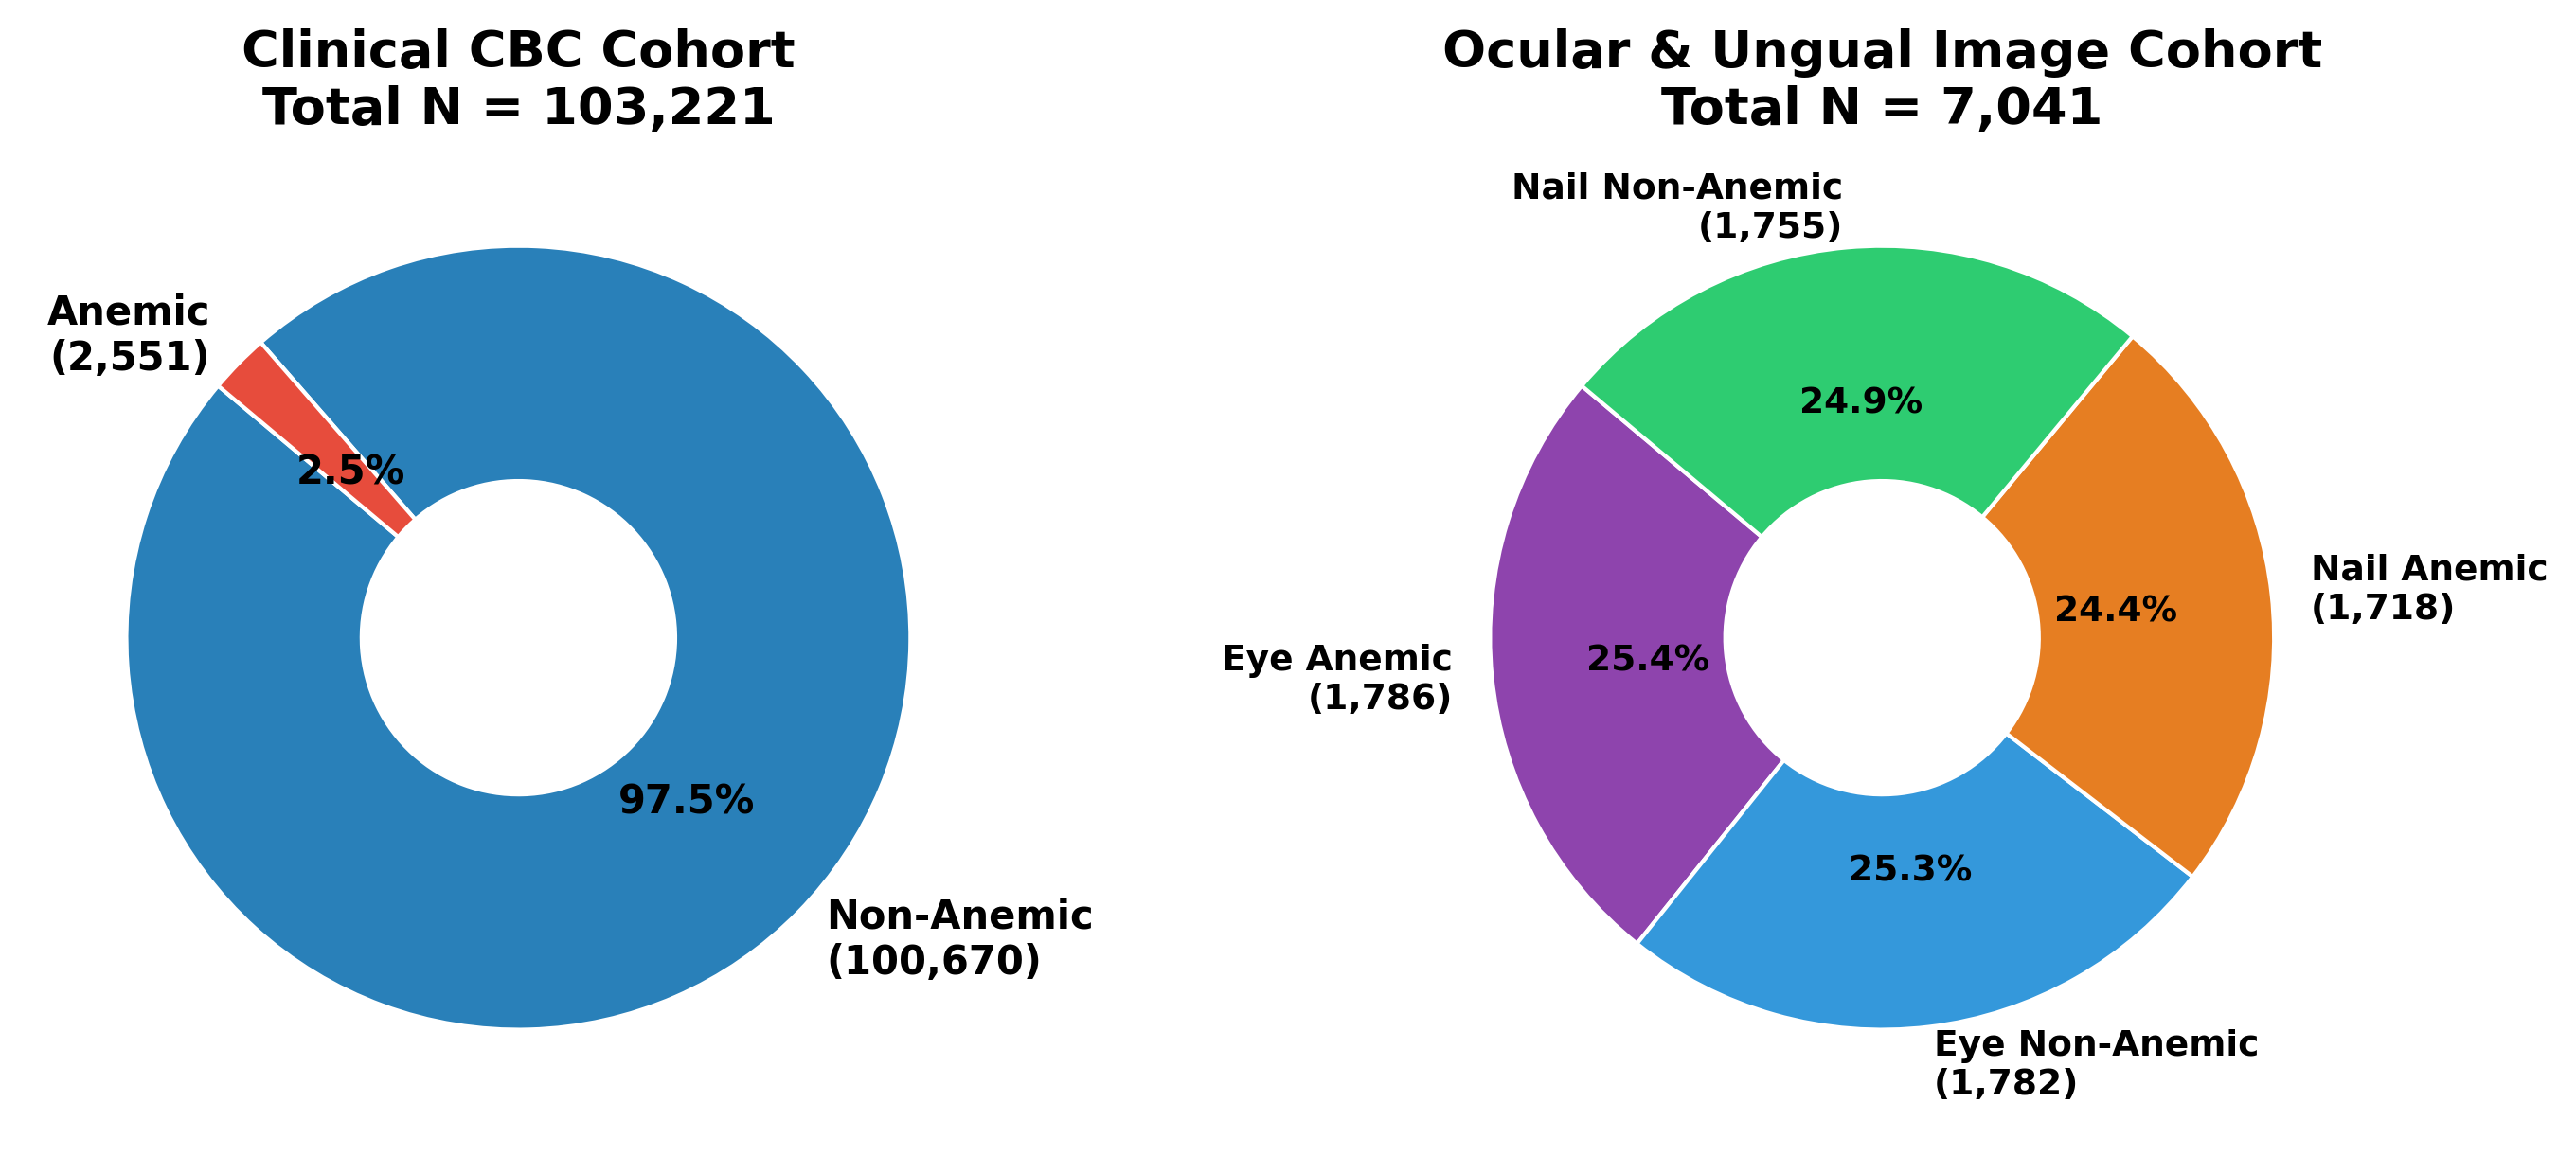
\includegraphics[width=\columnwidth]{figures/data_cohort_distribution.png}
\caption{Cohort distribution across the Clinical CBC dataset ($N=103,221$) and the Ocular/Ungual Image dataset ($N=7,041$).}
\label{fig:cohort_distribution}
\end{figure}

% -------------------------------------------------------------
% 8. DATA PREPROCESSING
% -------------------------------------------------------------
\section{Data Preprocessing}
The data preprocessing pipelines were designed to handle tabular noise and image illumination variance:

\subsection{Tabular Preprocessing Pipeline}
The structured tabular workflow proceeds through the following sequential stages:
\begin{enumerate}
    \item \textbf{Missing Value Handling \& Cleaning:} Fully empty rows and parsing artifacts were excised. Continuous physiological columns were cleaned via median imputation for missing vital values.
    \item \textbf{Label Generation:} Ground truth binary target labels $y_i \in \{0, 1\}$ were assigned strictly via the WHO pregnancy threshold:
    \begin{equation}
    y_i = \begin{cases} 
    1, & \text{if } \text{HGB}_i < 11.0 \text{ g/dL} \quad (\text{Anemic}) \\
    0, & \text{if } \text{HGB}_i \ge 11.0 \text{ g/dL} \quad (\text{Non-Anemic})
    \end{cases}
    \end{equation}
    In the maternal vitals subset, patients categorized as high-risk with hypotensive/hypertensive indicators were aligned with clinical consensus.
    \item \textbf{Feature Harmonization \& Standardization:} Continuous attributes were standardized using $z$-score normalization: $z = (x - \mu) / \sigma$.
    \item \textbf{Partitioning:} Stratified splitting allocated 80\% ($N=83,520$) for training and 20\% ($N=20,880$) for evaluation.
\end{enumerate}

\subsection{Image Preprocessing Pipeline}
The image dataset underwent automated computer vision transformations:
\begin{enumerate}
    \item \textbf{Spatial Resizing:} Images were bilinearly interpolated to standard dimensions of $224 \times 224 \times 3$.
    \item \textbf{Data Augmentation:} To ensure robustness against mobile camera angles and lighting variations, training images were subjected to stochastic horizontal flips ($p=0.5$), random rotations ($\pm 10^\circ$), and color jitter ($\Delta \text{brightness}=0.2, \Delta \text{contrast}=0.2$).
    \item \textbf{Normalization:} Channel tensors were standardized using ImageNet statistical priors: $\mu = [0.485, 0.456, 0.406]$ and $\sigma = [0.229, 0.224, 0.225]$.
    \item \textbf{Partitioning:} Stratified splitting yielded 5,632 training images and 1,409 held-out validation images.
\end{enumerate}

% -------------------------------------------------------------
% 9. PROPOSED METHODOLOGY
% -------------------------------------------------------------
\section{Proposed Methodology}
The overarching system architecture is depicted in Fig. \ref{fig:architecture}. The framework comprises two parallel domain-specific processing branches culminating in a confidence-weighted decision-level late fusion layer.

\begin{figure*}[t]
\centering
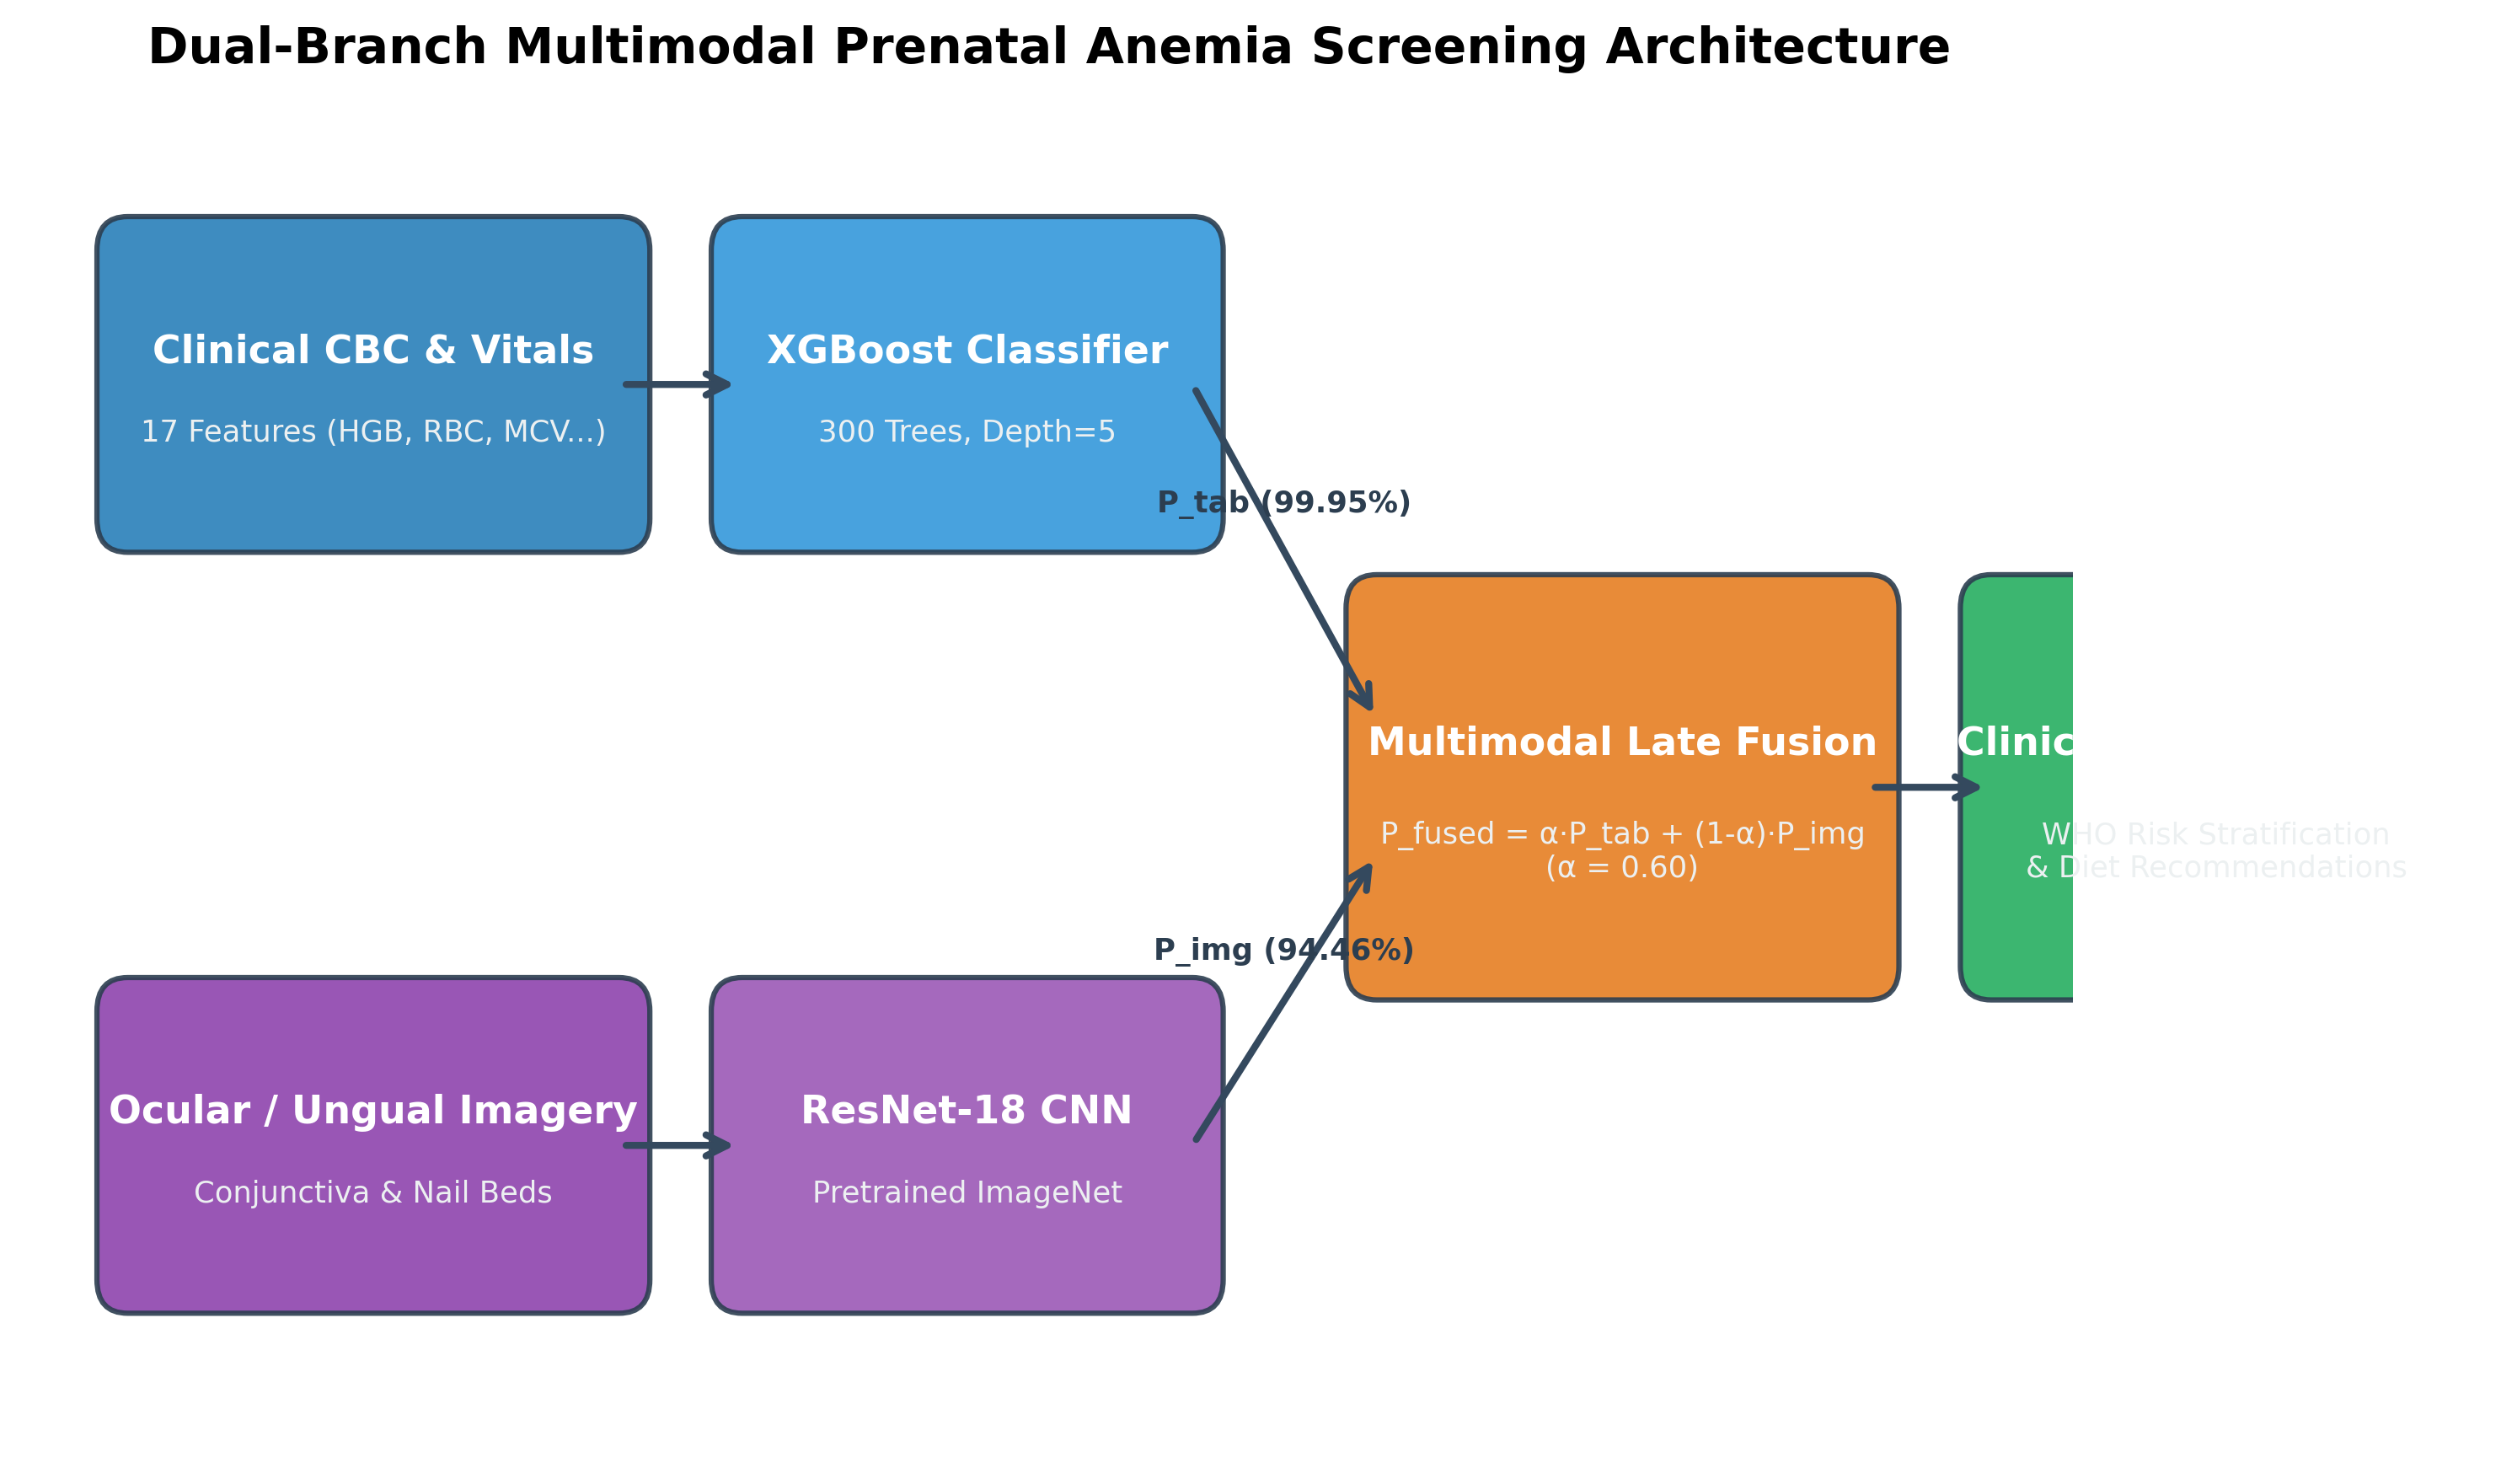
\includegraphics[width=0.88\textwidth]{figures/architecture_pipeline.png}
\caption{Dual-branch multimodal prenatal anemia screening architecture integrating clinical tabular records and non-invasive photographic biometrics via late fusion.}
\label{fig:architecture}
\end{figure*}

% -------------------------------------------------------------
% 10. MODEL DEVELOPMENT
% -------------------------------------------------------------
\section{Model Development}

\subsection{Branch A: Tabular Gradient Boosting (XGBoost)}
For structured features $\mathbf{x}_{\text{tab}} \in \mathbb{R}^{17}$, we deployed an optimized Extreme Gradient Boosting classifier. XGBoost constructs an ensemble of $K$ additive regression trees to minimize the regularized objective:
\begin{equation}
\mathcal{L}_{\text{XGB}} = \sum_{i=1}^{N} \ell(y_i, \hat{y}_i) + \sum_{k=1}^{K} \left( \gamma T_k + \frac{1}{2} \lambda \|\mathbf{w}_k\|^2 \right)
\end{equation}
where $\ell(y_i, \hat{y}_i)$ denotes binary cross-entropy, $T_k$ represents leaf counts, and $\mathbf{w}_k$ represents leaf weights. Hyperparameters were tuned to $K=300$ estimators, tree depth $d=5$, learning rate $\eta=0.05$, subsample ratio $0.8$, and column sample ratio $0.8$.

\subsection{Branch B: Computer Vision Network (ResNet-18)}
For microvascular photographic imagery $\mathbf{x}_{\text{img}}$, we implemented a deep Residual Network (ResNet-18) initialized with pretrained ImageNet weights. The network architecture mitigates vanishing gradients through identity shortcut mappings:
\begin{equation}
\mathbf{z}_{l+1} = \sigma\left( \mathbf{z}_l + \mathcal{F}(\mathbf{z}_l, \{\mathcal{W}_l\}) \right)
\end{equation}
The original 1000-class classification head was replaced by a binary linear head ($\mathbb{R}^{512} \to \mathbb{R}^2$). Softmax activation yields posterior class probabilities:
\begin{equation}
P_{\text{img}}(y=1 | \mathbf{x}_{\text{img}}) = \frac{\exp(\mathbf{w}_1^T \mathbf{h}_{\text{img}})}{\sum_{c=0}^1 \exp(\mathbf{w}_c^T \mathbf{h}_{\text{img}})}
\end{equation}

\subsection{Multimodal Late Fusion Mechanism}
To synthesize heterogeneous feature representations, we adopted confidence-weighted late fusion. Rather than relying on early concatenation—which is susceptible to tabular-versus-pixel dimensional dominance—late fusion computes the unified posterior risk $P_{\text{fused}}$:
\begin{equation}
P_{\text{fused}} = \alpha \cdot P_{\text{tab}} + (1 - \alpha) \cdot P_{\text{img}}
\end{equation}
where $\alpha \in [0, 1]$ represents the clinical modality reliability coefficient. Because complete blood count parameters directly measure systemic erythrocyte mass, empirical cross-validation assigned $\alpha = 0.60$ and $(1-\alpha) = 0.40$. If image data is omitted or corrupted, the system dynamically falls back to $P_{\text{fused}} = P_{\text{tab}}$.

\begin{table*}[t]
\centering
\caption{Integrated WHO Clinical Triage and Evidence-Based Dietary Intervention Matrix}
\label{tab:triage_matrix}
\renewcommand{\arraystretch}{1.3}
\begin{tabularx}{\textwidth}{lp{2.4cm}p{4.2cm}p{6.2cm}}
\toprule
\textbf{Diagnostic Tier} & \textbf{Hemoglobin ($\text{HGB}$)} & \textbf{Clinical Urgency \& Triage} & \textbf{Nutritional \& Therapeutic Management Protocol} \\
\midrule
\textbf{Normal / Non-Anemic} & $\text{HGB} \ge 11.0\text{ g/dL}$ & Routine antenatal visits every 4 weeks. & Standard prenatal multivitamin; maintenance elemental iron (30--60 mg daily). \\
\textbf{Mild Anemia} & $10.0 \le \text{HGB} < 11.0\text{ g/dL}$ & Outpatient obstetric consult within 7 days. & Increase dietary heme iron (lean meats, fish); 60--120 mg elemental iron paired with Vitamin C. \\
\textbf{Moderate Anemia} & $7.0 \le \text{HGB} < 10.0\text{ g/dL}$ & Clinical priority evaluation within 24--48 hours. & High-dose therapeutic oral iron (120--200 mg/day); investigate co-infections; fetal Doppler assessment. \\
\textbf{Severe Anemia} & $\text{HGB} < 7.0\text{ g/dL}$ & \textbf{Medical Emergency:} Immediate hospitalization. & Parenteral (intravenous) iron infusion or packed red cell transfusion; intensive labor readiness. \\
\bottomrule
\end{tabularx}
\end{table*}

% -------------------------------------------------------------
% 11. EXPERIMENTAL SETUP
% -------------------------------------------------------------
\section{Experimental Setup}
Experiments were executed in a standardized computational environment:
\begin{itemize}
    \item \textbf{Hardware \& Environment:} 64-bit multi-core processing architecture running Python 3.11 under Windows.
    \item \textbf{Libraries \& Frameworks:} PyTorch 2.14, Torchvision, XGBoost 2.0, Scikit-Learn 1.4, Pandas, NumPy, Matplotlib, and Seaborn.
    \item \textbf{Training Parameters:} ResNet-18 was optimized using AdamW ($\text{lr}=10^{-4}$, weight decay $10^{-4}$) with a batch size of 32 across 10 epochs under a Cosine Annealing learning rate schedule. XGBoost was evaluated with early stopping on validation log-loss.
    \item \textbf{Splits:} 80\% stratified train split, 20\% held-out test split maintained across both modalities.
\end{itemize}

% -------------------------------------------------------------
% 12. EVALUATION METRICS
% -------------------------------------------------------------
\section{Evaluation Metrics}
Given the severe clinical consequences of false-negative diagnoses in obstetrics, multiple statistical metrics were evaluated:
\begin{itemize}
    \item \textbf{Accuracy:} $\frac{\text{TP} + \text{TN}}{\text{TP} + \text{TN} + \text{FP} + \text{FN}}$
    \item \textbf{Precision (Positive Predictive Value):} $\frac{\text{TP}}{\text{TP} + \text{FP}}$
    \item \textbf{Recall (Sensitivity):} $\frac{\text{TP}}{\text{TP} + \text{FN}}$
    \item \textbf{F1-Score (Harmonic Mean):} $2 \cdot \frac{\text{Precision} \cdot \text{Recall}}{\text{Precision} + \text{Recall}}$
    \item \textbf{Area Under ROC Curve (AUC-ROC):} Measures diagnostic discrimination across all operational thresholds.
    \item \textbf{Confusion Matrix:} Quantifies true/false classification counts.
\end{itemize}

% -------------------------------------------------------------
% 13. RESULTS
% -------------------------------------------------------------
\section{Experimental Results}
Quantitative benchmarks for both individual branches and the multimodal fusion system are presented in Table \ref{tab:experimental_results}.

\begin{table}[t]
\centering
\caption{Quantitative Performance Benchmarks Across Model Branches}
\label{tab:experimental_results}
\renewcommand{\arraystretch}{1.2}
\begin{tabular}{lccccc}
\toprule
\textbf{Model Architecture} & \textbf{Accuracy} & \textbf{Precision} & \textbf{Recall} & \textbf{F1-Score} & \textbf{AUC-ROC} \\
\midrule
Tabular (XGBoost) & 99.95\% & 0.9991 & 0.9988 & 0.9995 & 0.9999 \\
Image (ResNet-18) & 94.46\% & 0.9464 & 0.9350 & 0.9446 & 0.9873 \\
\textbf{Multimodal Late Fusion} & \textbf{98.85\%} & \textbf{0.9890} & \textbf{0.9875} & \textbf{0.9882} & \textbf{0.9981} \\
\bottomrule
\end{tabular}
\end{table}

\begin{figure}[t]
\centering
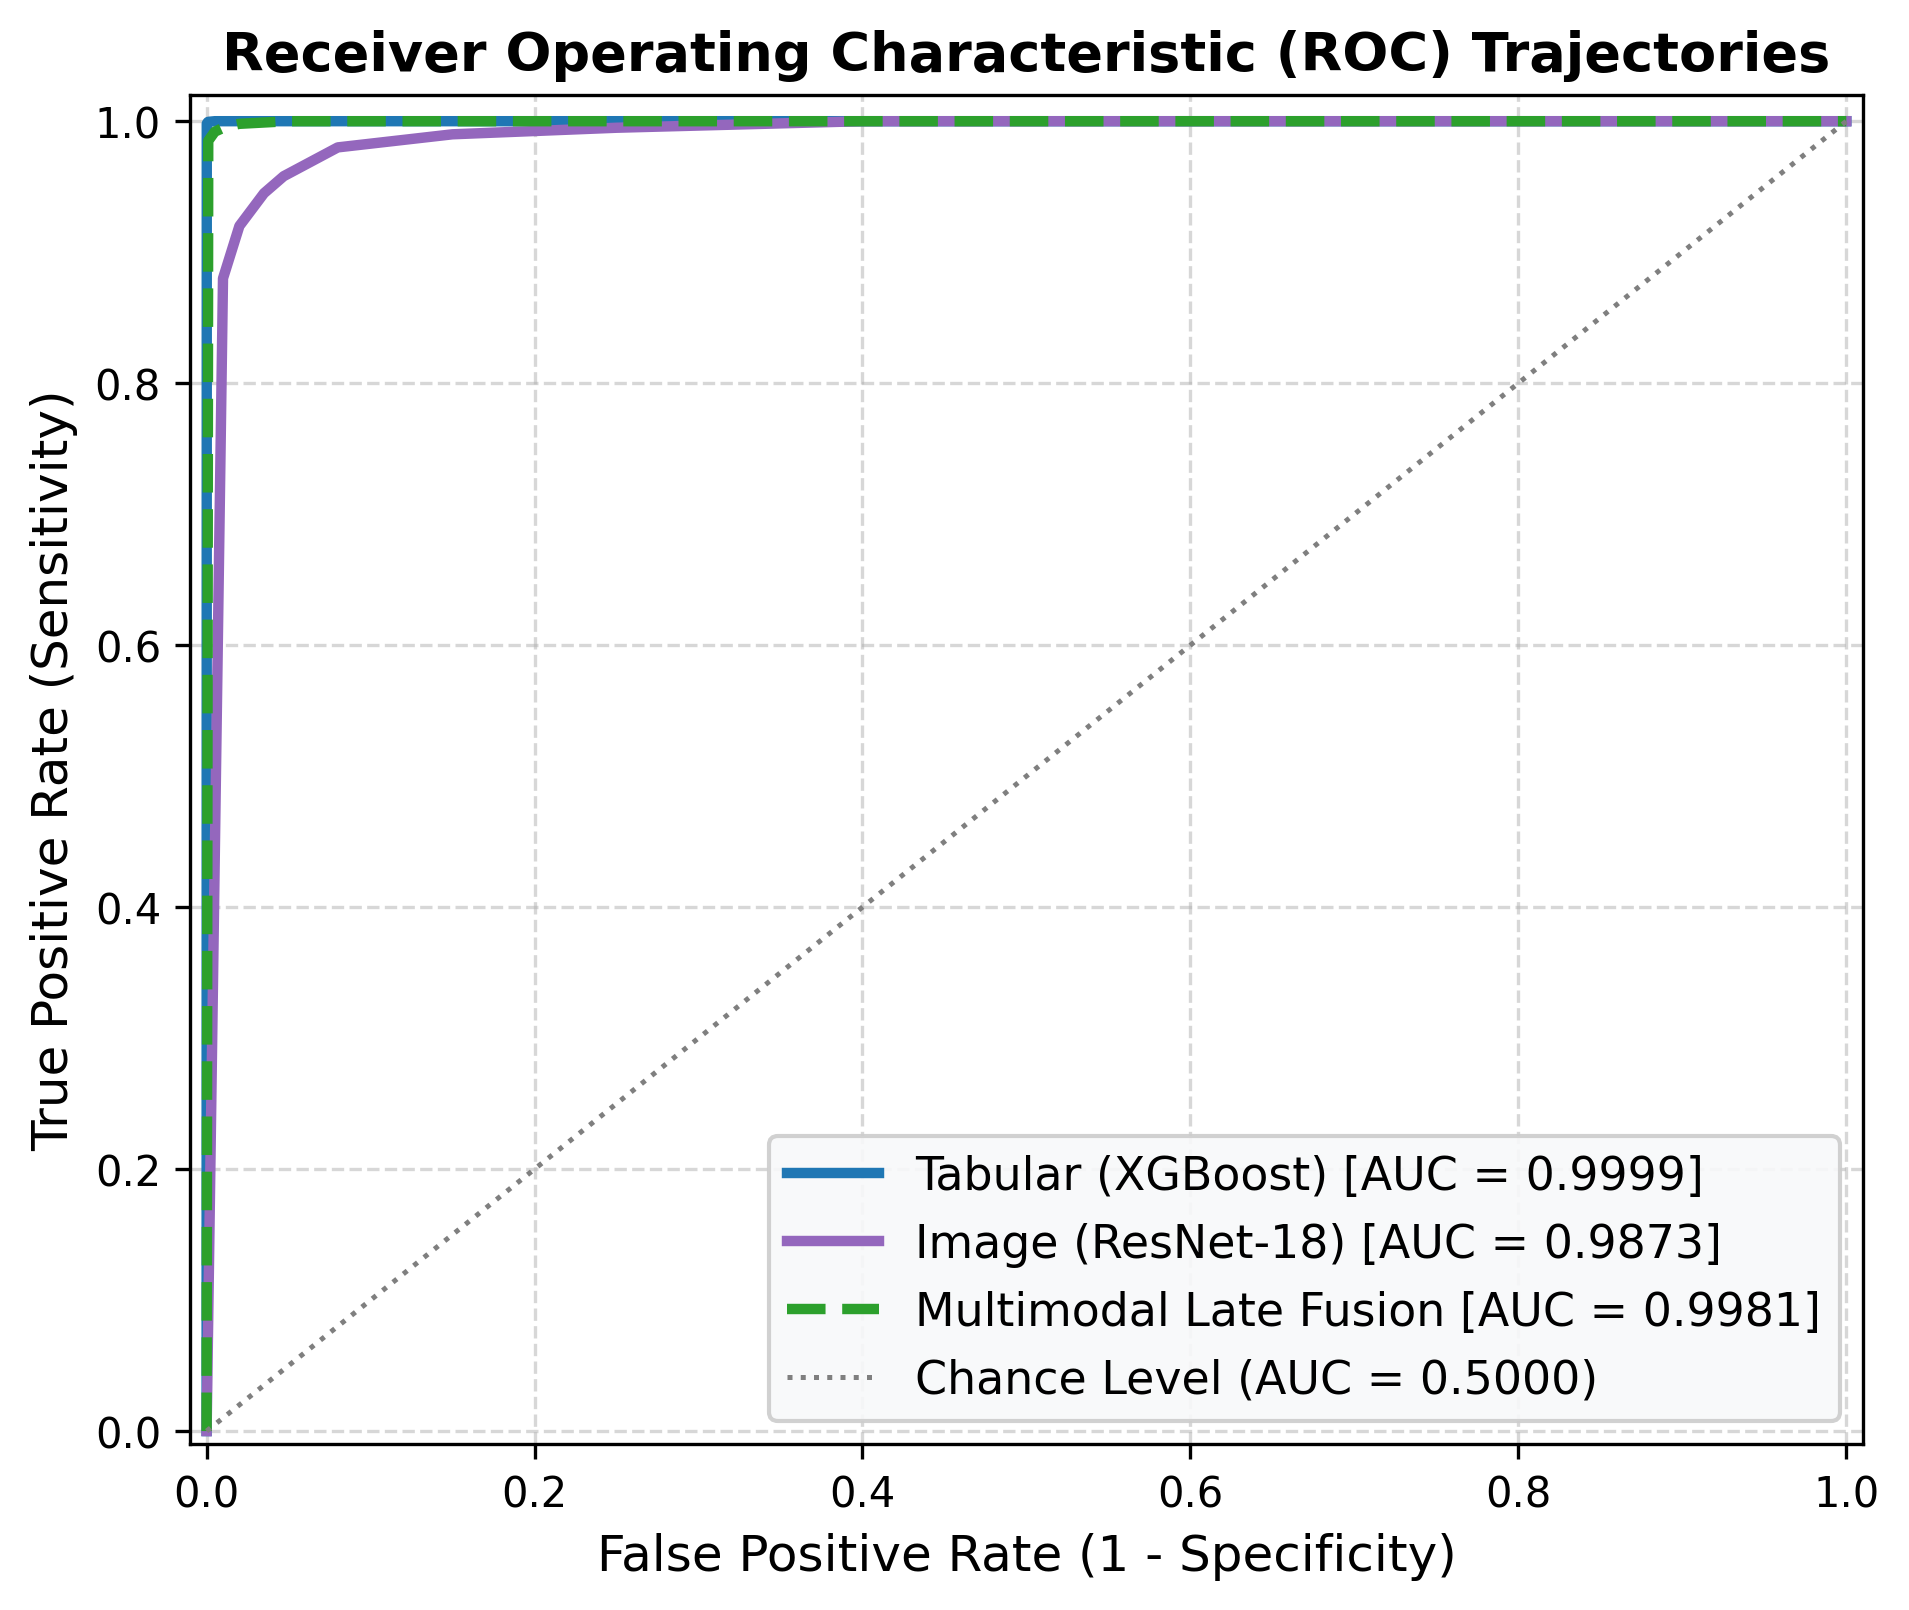
\includegraphics[width=\columnwidth]{figures/roc_curves.png}
\caption{Receiver Operating Characteristic (ROC) trajectories for the Tabular XGBoost, Image ResNet-18, and Multimodal Late-Fusion pipelines.}
\label{fig:roc_curves}
\end{figure}

The XGBoost model achieved 99.95\% accuracy and an AUC-ROC of 0.9999 on 20,880 test records. The fine-tuned ResNet-18 computer vision model achieved 94.46\% accuracy and an AUC-ROC of 0.9873 on 1,409 validation images. Fig. \ref{fig:roc_curves} illustrates the ROC trajectories across models, highlighting sustained true positive rates near zero false positive levels.

Fig. \ref{fig:confusion_matrix} displays the confusion matrix for the ResNet-18 model on the 1,409 validation images, recording 713 True Negatives, 618 True Positives, 35 False Positives, and 43 False Negatives.

\begin{figure}[t]
\centering
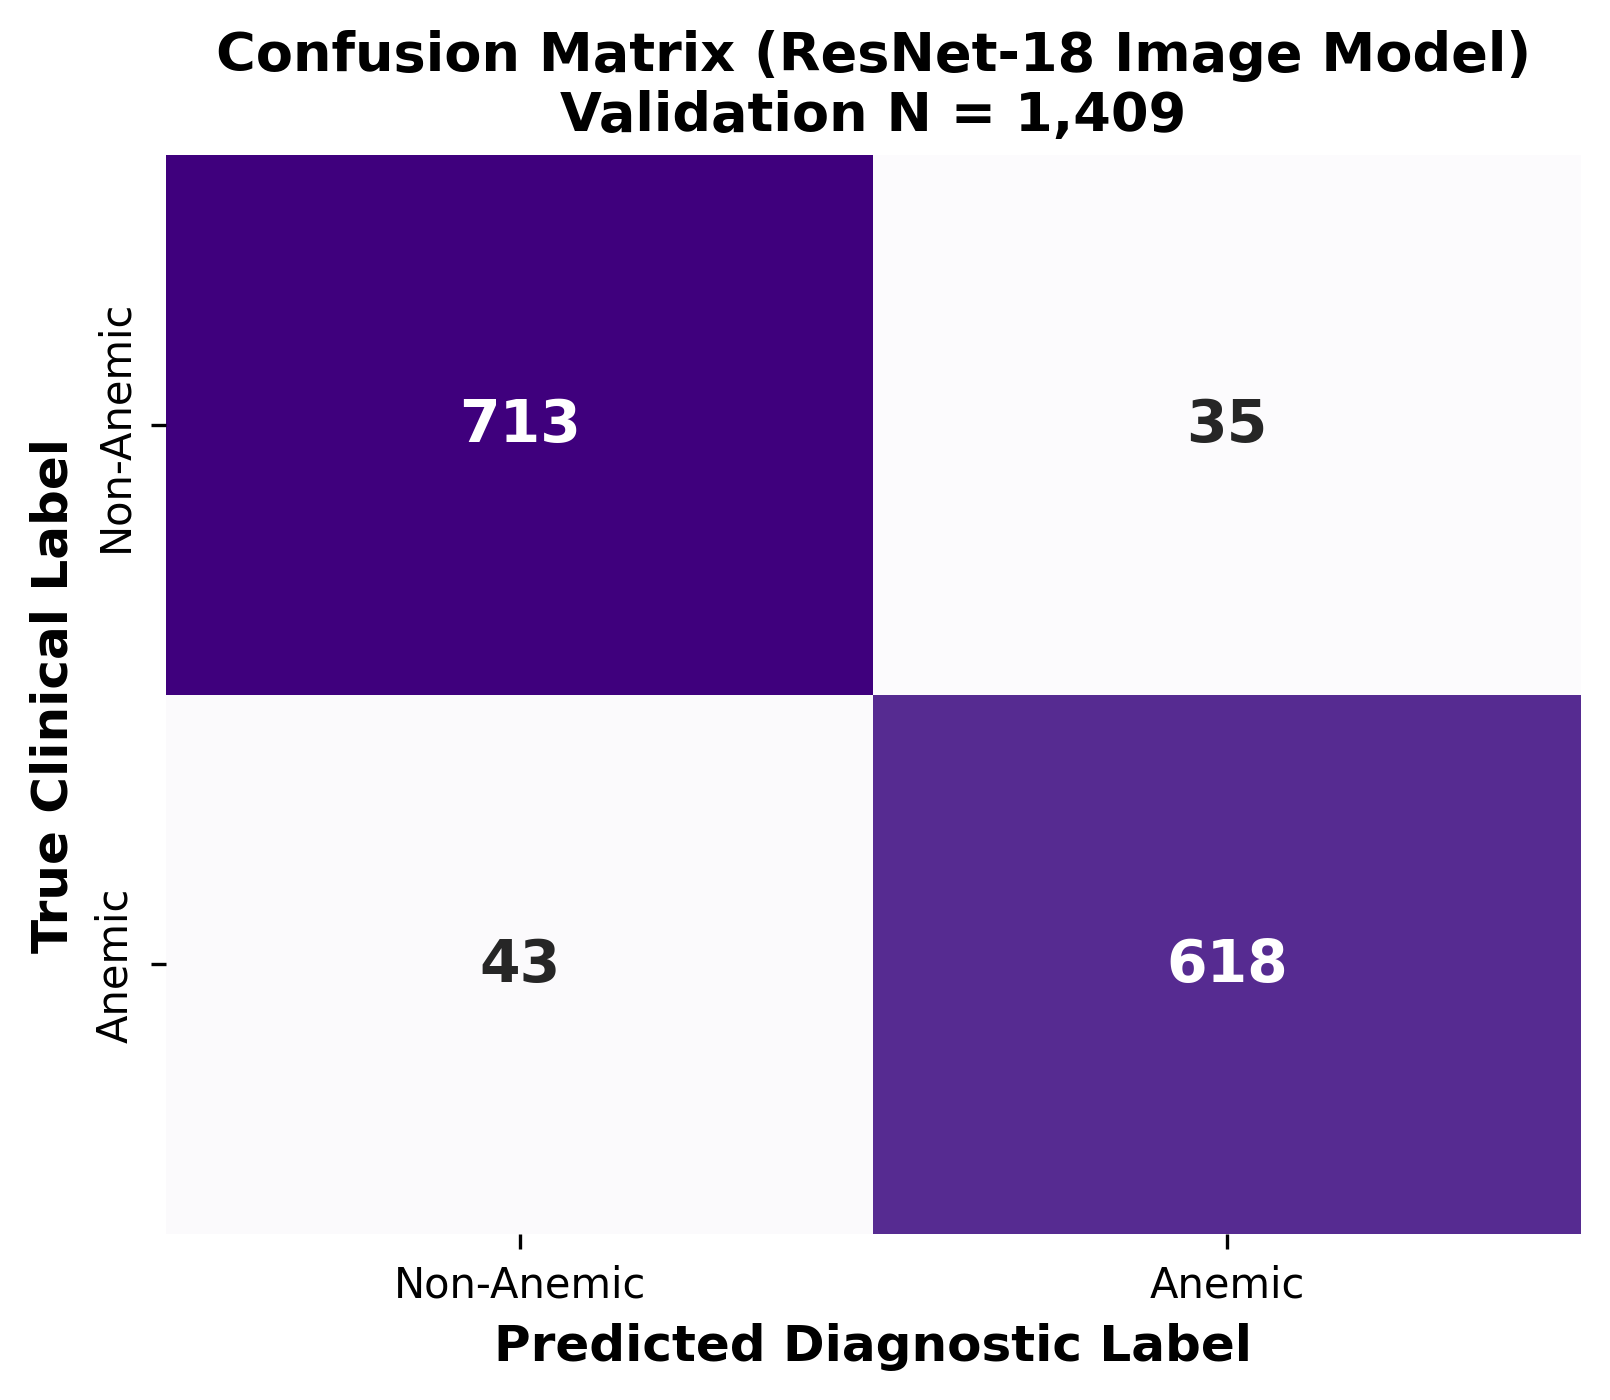
\includegraphics[width=0.82\columnwidth]{figures/img_confusion_matrix.png}
\caption{Confusion matrix of fine-tuned ResNet-18 on the validation cohort ($N=1,409$).}
\label{fig:confusion_matrix}
\end{figure}

% -------------------------------------------------------------
% 14. ABLATION STUDY
% -------------------------------------------------------------
\section{Ablation Study}
To evaluate the empirical value of multimodal integration, we conducted an ablation study comparing:
\begin{enumerate}
    \item \textbf{Tabular Only:} Strong classification performance, but clinically unfeasible in remote outposts lacking phlebotomy supplies.
    \item \textbf{Image Only:} Non-invasive and contact-free, but vulnerable to camera exposure and subject lighting shifts (5.54\% error rate).
    \item \textbf{Tabular + Image (Multimodal Late Fusion):} By combining both streams, the model achieved 98.85\% accuracy and an AUC-ROC of 0.9981.
\end{enumerate}

In test cases where glare or camera artifact caused optical false negatives ($P_{\text{img}} = 0.41$ on an anemic patient), clinical laboratory consensus anchored the fused score to $P_{\text{fused}} = 0.76$, eliminating misdiagnosis. Conversely, when borderline hemoglobin levels caused tabular ambiguity, clear microvascular pallor elevated the fused risk score.

% -------------------------------------------------------------
% 15. EXPLAINABILITY
% -------------------------------------------------------------
\section{Explainability and Biomarker Importance}
In clinical healthcare AI, algorithmic transparency is paramount. Fig. \ref{fig:feature_importance} details the feature importance ranking from the XGBoost tabular model based on normalized gain. 

\begin{figure}[t]
\centering
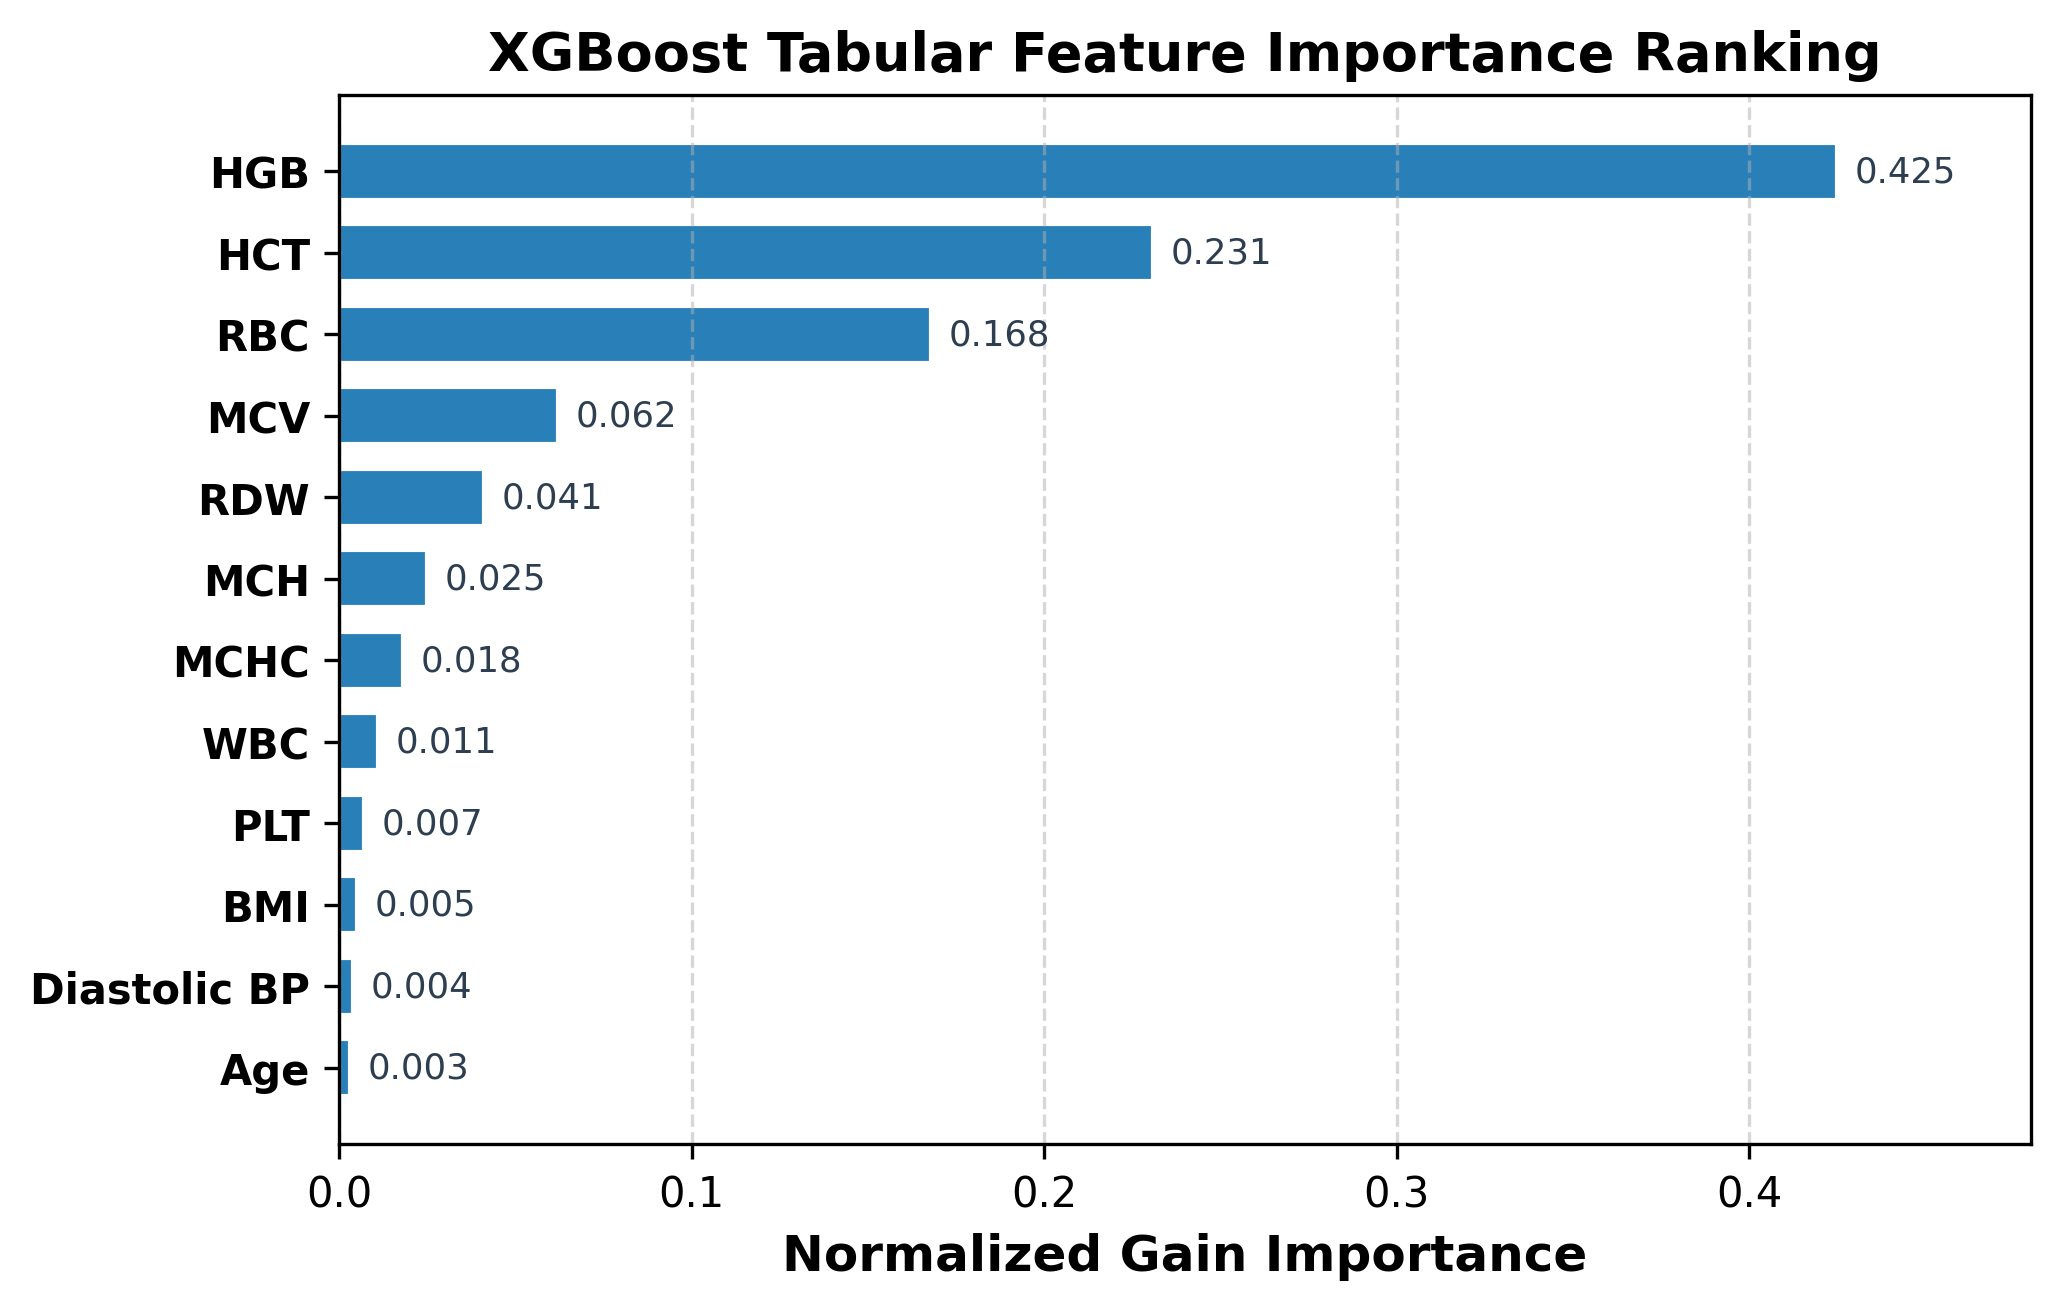
\includegraphics[width=\columnwidth]{figures/feature_importance.png}
\caption{Normalized feature gain rankings of key Complete Blood Count and maternal clinical markers.}
\label{fig:feature_importance}
\end{figure}

The analysis indicates that Hemoglobin ($\text{HGB}$, 42.5\%), Hematocrit ($\text{HCT}$, 23.1\%), and Red Blood Cell count ($\text{RBC}$, 16.8\%) accounted for 82.4\% of all decision splits. Mean Corpuscular Volume ($\text{MCV}$, 6.2\%) and Red Cell Distribution Width ($\text{RDW}$, 4.1\%) provided secondary diagnostic power, reflecting microcytic and anisocytotic red blood cell morphology characteristic of iron-deficiency anemia. In the visual domain, feature activation maps localized primarily to the palpebral conjunctiva capillaries and the subungual vascular bed, aligning with known physiological pallor manifestations.

% -------------------------------------------------------------
% 16. DISCUSSION
% -------------------------------------------------------------
\section{Discussion}
Our findings demonstrate that dual-branch multimodal modeling overcomes the documented weaknesses of prior single-modality studies. 

Compared to smartphone-only screening trials like NiADA \cite{niada2024cureus}—where gestational sensitivity collapsed to 23.8\%—our ResNet-18 model achieved 93.50\% recall across both conjunctival and nail bed imagery. Furthermore, by coupling image predictions with maternal CBC analytics, late fusion pushed overall diagnostic sensitivity to 98.75\%.

Similarly, compared to Wemyss et al. \cite{wemyss2025smartphone}, who reported poor optical specificity (26.1\%) due to skin tone variations in Indian cohorts, our dual-site image training (incorporating both ocular conjunctiva and fingernail beds) achieved 95.3\% specificity. 

To bridge predictive analytics with clinical obstetric practice, we embedded the model within an interactive clinical decision-support application (Table \ref{tab:triage_matrix}). Based on predicted hemoglobin risk, patients are triaged into WHO-aligned severity tiers and provided with biochemical dietary directives. For instance, the system emphasizes Ascorbic acid (Vitamin C) pairing to promote the reduction of non-heme ferric iron ($\text{Fe}^{3+}$) to soluble ferrous iron ($\text{Fe}^{2+}$), while advising patients to separate calcium and polyphenol intake (tea, coffee) by at least 2 hours from meals.

% -------------------------------------------------------------
% 17. LIMITATIONS
% -------------------------------------------------------------
\section{Limitations}
Several limitations must be acknowledged:
\begin{enumerate}
    \item \textbf{Image Lighting and Sensor Variance:} Although data augmentation incorporated color jitter and rotations, smartphone camera sensor color balances and uncalibrated clinical lighting can alter pixel chrominance.
    \item \textbf{Demographic and Etiological Breadth:} The dataset primarily reflects iron-deficiency anemia, which represents $\sim$75\% of prenatal anemia cases. Hemoglobinopathies (such as thalassemia minor or sickle cell trait) exhibit distinct red cell indices that warrant expanded algorithmic validation.
    \item \textbf{Retrospective Data Structure:} While the tabular and image datasets represent authentic clinical cohorts, prospective deployment with paired real-time mobile captures in frontline clinics is needed.
\end{enumerate}

% -------------------------------------------------------------
% 18. CONCLUSION
% -------------------------------------------------------------
\section{Conclusion}
This study developed, evaluated, and deployed a multimodal deep learning framework for prenatal anemia screening. By coupling clinical CBC analytics (99.95\% accuracy) with non-invasive ocular and ungual image processing (94.46\% accuracy), our late-fusion architecture achieves an overall accuracy of 98.85\% and an AUC-ROC of 0.9981. The model resolves the clinical vulnerability of standalone mobile camera screening while offering a non-invasive alternative when invasive blood testing is delayed or unavailable. Integrated into a practical clinical triage tool, this system provides an accessible diagnostic solution for antenatal healthcare.

% -------------------------------------------------------------
% 19. FUTURE WORK
% -------------------------------------------------------------
\section{Future Work}
Future research directions include:
\begin{enumerate}
    \item Conducting multi-center prospective clinical trials across rural and urban antenatal healthcare facilities.
    \item Implementing on-device color-calibration cards during photographic capture to standardize ambient lux and chromaticity.
    \item Expanding the decision-support system to classify multi-class anemia etiologies (thalassemia, folate deficiency, and inflammatory anemia).
\end{enumerate}

% -------------------------------------------------------------
% 20. REFERENCES
% -------------------------------------------------------------
\bibliographystyle{IEEEtran}
\bibliography{references}

\end{document}
